\chapter{Implementaci\'{o}}
\label{cha:implementation}
En aquest capítol es descriuen les tecnologies estudiades i aplicades per implementar el disseny anteriorment descrit.

\section{Estudi previ de les tecnologies}
En aquesta secci\'{o} es far\'{a} una descripci\'{o} de les tecnologies estudiades per tal de poder realitzar aquest projecte. 

\subsection{\textit{Framework} a mida}
En un principi \'{e}s va valorar la possibilitat de desenvolupar tot un nou \textit{framework} per la implementaci\'{o} del projecte. Les tecnologies emprades son PHP com a llenguatge de programaci\'{o} i MySQL com a motor de bases de dades.
\paragraph{Avantatges}
\begin{itemize} 
\item La principal avantatge \'{e}s el control total de la implantaci\'{o} de tots els processos i tecnologies.
\end{itemize} 

\paragraph{Desavantatges}
\begin{itemize} 
\item Desenvolupament extremadament lent.
\item Re-inventar la roda quan no \'{e}s necessari.
\end{itemize} 

\subsection{\textit{Codeigniter}}
Codeigniter \'{e}s un \textit{framework} per a desenvolupament web r\`{a}pid amb PHP.\cite{codeigniter} Usa el patr\'{o} ''active record' per la gesti\'{o} d'emmagatzematge de dades.\cite{activerecord}
\paragraph{Avantatges}
\begin{itemize}
\item Corba d'aprenentatge rapida.
\item Desenvolupament r\`{a}pid.
\item \'{E}s patr\'{o} MVC.
\end{itemize}

\paragraph{Desavantatges}
\begin{itemize}
\item No compleix tots el requisits de disseny de patrons especificat.
\item No inclou \textit{templating}
\item Dificultat en segregar la l\`{o}gica de la presentaci\'{o}.
\end{itemize}

\subsection{\textit{Symfony2}}
\textit{Symfony2} \'{e}s un HTTP \textit{framework} per a PHP. Nativament implementa una variaci\'{o} del Model-Vista-Controlador amb controlador frontal amb injecci\'{o} de depencies a la capa de serveis.\cite{symfony}

\paragraph{Avantatges}
\begin{itemize}
\item Altament configurable.
\item Compleix tots els requisits de dissenys de patrons especificat.
\item Alt rendiment
\end{itemize}

\paragraph{Desavantatges}
\begin{itemize}
\item Corba d'aprenentatge alta.
\end{itemize}

\section{Implementaci\'{o}}
El \itemit{framework} escollit ha sigut \textit{Symfony2}. A continuaci\'{o} es dona una visi\'{o} general de les tecnologies.

\subsection{\textit{Symfony2}}
Arquitectonicament, \textit{Symfony2} estructura el codi en \textit{Bundles}, similar als paquets de JAVA. Els \textit{bundles} son un conjunt de serveis, entitats i recursos independents entre si. Els \textit{bundles} implementats son:
\begin{itemize}
\item \textit{Bundle} de usuaris: UserBundle. Paquet de serveis, vistes i recursos per usuaris. S'ha utilitzat un paquet de \textit{Symfony2}: FOSUserBundle \cite{fosuserbundle}. S'ha fet una extensi\'{o} del paquet per implementar la gesti\'{o} de rols i grups.
\item \textit{Bundle} de matrius: MatrixBundle. Paquet de serveis, vistes i recursos per les matrius.
\item \textit{Bundle} de trainings: TrainingBundle. Paquet de serveis, vistes i recursos per els entrenaments.
\item \textit{Bundle} de serveis webs: ApiBundle. Paquet de serveis,vistes i recursos per la API JSON Restful. 
\item \textit{Bundle} de predicci\'{o}: PredictionBundle. Paquet de serveis, vistes i recursos per les matrius de prediccions.
\end{itemize}

\subsection{Gesti\'{o} de depend\`{e}ncies} 
\textit{Symfony2} utilitza \textit{Composer} per la gesti\'{o} de depend\`{e}ncies.\cite{composer} \textit{Composer} \'{e}s un gestor de dependencies a nivell d'aplicaci\'{o}. Les depend\`{e}ncies son:
\begin{itemize}
\item Jquery: llibreria Javascript que s'executa en el costat client per enriquir les interfícies. Simplifica la manera de interaccionar amb els documents HTML i la simplifica la manera de manipular l'arbre DOM.\cite{jquery}
\item FOSUserBundle: paquet per a \textit{Symfony} per la gesti\'{o} de usuaris.\cite{fosuserbundle}
\item Bootstrap: \texit{framework} pel \textit{front-end} desenvolupat per Twitter. Implementa nous estàndards com HTML5 i CSS3. Permet el desenvolupament d'interf\'{i}cies de manera r\`{a}pida i usables suportades per múltiples navegadors.
\item RestBundle: paquet per Symfony per desenvolupar llibreries API JSON Restful.\cite{apijson}
\item Symfony FS: paquet per gestionar sistema de fitxers.
\item Doctrine Fixtures: paquet per gestionar la inserci\'{o} controlada de dades a la base de dades.
\item TWIG: motor de plantilles per a PHP.\cite{twig}
\item Doctrine: ORM pel mapatge de dades, usant MySQL.\cite{mysql}
\item Sistema de cues: projecte desenvolupat per Miguel Ibero conjuntament amb aquest per la execució de Ichnaea.
\end{itemize}

\subsection{Recursos}
La estructura de recursos de la aplicaci\'{o} \'{e}s la següent:\\

\begin{tabular}{| l | l |}
\hline
Matrius     & matrix/(id) \\ \hline
Entrenamens & matrix/(id)/training/(id) \\ \hline
Prediccions & matrix/(id)/training/(id)/prediction/(id) \\ \hline
\end{tabular}\\

S'ha emprat aquesta estructura de recursos degut a les dependències entre les diferents entitats. Un entrenament dep\'{e}n d'una matriu i una predicci\'{o} dep\'{e}n d'un entrenament.

\section{API: llibreria de serveis web}
S'ha desenvolupat una llibreria API JSON RESTful per donar resposta a les funcionalitats asíncrones de les interfícies.\cite{apijson} S'ha emprat aquesta tecnologia per la escal.labilitat que aporta i perquè en un futur es pugui aprofitar el desenvolupament d'aquesta amb la integració d'altres tipus client, com poden ser aplicacions mòbils o altres serveis.\\

La arquitectura RESTful aprofita al màxim el protocol HTTP per establir dades i actualment s'usen per donar funcionalitats asincrones a les interficies(mirar \ref{sec:dessigninterfaces}).

Les operacions, els recursos i el paràmetres implementats son:\\
\begin{figure}[H]
  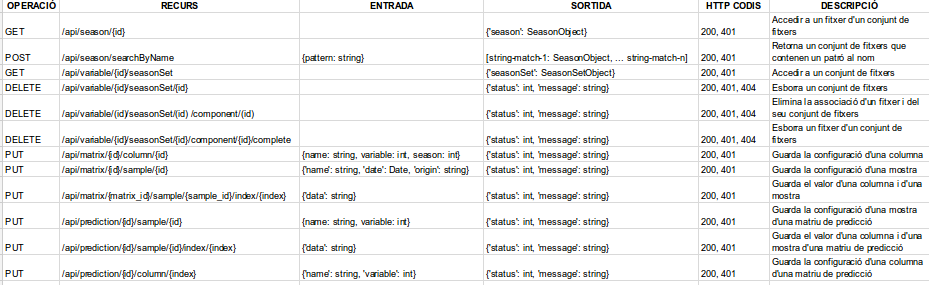
\includegraphics[scale=0.5]{img/implementation/apirestul.png}
  \caption{Operacions de serveis web}
  \label{fig:dessignpatters}
\end{figure}
On:
\begin{itemize}
\item Operació \'{e}s el mètode HTTP.
\item Recurs \'{e}s el identificador del recurs.
\item Entrada \'{e}s l'objecte JSON d'entrada de la operació.
\item Sortida \'{e}s l'objecte JSON de sortida de la operació.
\item HTTP Codi son els codis HTTP que retornen.\cite{listhttpcodis}
\end{itemize}

Totes les operacions estan securitzades per \textit{cookies}\cite{cookies} i per sessió per identificar i validar a l'usuari.\cite{sessions}

\section{Integraci\'{o} amb el sistema de cues RabbitMQP}
\subsection{Introducci\'{o} a l'arquitectura de cues: AMQP}
\label{sec:queue_system_overview}
L'est\`{a}ndard AMQP (''Advanced Message Queuing Protocol'') \'{e}s un protocol d'est\`{a}ndard obert en la capa d'aplicacions d'un sistema de comunicació. Les característiques que defineixen al protocol AMQP son la orientació a missatges, encuament(''queuing''), enrutament i exactitud, entre altres com,per exemple, la seguretat o les subscripcions.\cite{amqp}\\

AMQP defineix una s\`{e}rie d'entitats. Des de la perspectiva de la interconnexió les m\'{e}s rellevants son:
\begin{itemize}
\item El corredor de missatges: un servidor on els clients AMQP es connecten usant el protocol AMQP. Els corredores de missatges poden executar-se en un entorn distribuït, però aquesta capacitat \'{e}s espec\'{i}fica de la implementació.
\item Usuari: un usuari \'{e}s una entitat amb credencial pot ser autoritzat a connectar-se a un corredor.
\item Connexió: una connexi\'{o} f\'{i}sica, usant per exemple TCP/IP, entre el corredor i l'usuari.
\item Clients: productors i consumidors. \'{E}s un model de comunicacio con el productor \'{e}s un proces emissor  i el consumidor \'{e}s un proces receptor.\cite{messaging}
\end{itemize}

\textbf{RabbitMQ} \'{e}s un \textit{software} que implementa aquest protocol. El sistema de cues est\'{a} implementat com a Projecte de Final de Carrera de Miguel Ibero i ofereix una llibreria per la seva integració.\\

Per la integració amb el sistema amb cues s'ha desenvolupat:
\begin{itemize}
\item Gestionar la dependència.
\item Desenvolupar el consumidors.
\end{itemize}

\subsection{Consumidors i gesti\'{o} de resultats}
Els consumidors en el protocol de missatgeria son els processos receptors de missatges emesos per els productors. Les respostes de les execucions de Ichnaea  (mirar la figura \ref{dessign:archsoftware}) les rep el consumidor. \\

\textit{Symfony2} permet crear comandes CLI per crear processos. Els consumidors necessiten ser processos ''stand-alone''(aut\'{o}noms) que escoltin les sortides i consumeixin els resultats de la cua. \\

L'esquelet d'una comanda per aquests consumidors actualment \'{e}s:
\begin{lstlisting}
class ConsumerCommand extends ContainerAwareCommand
{
	//Definicio de la comanda
	protected function configure()
	{
		$this
		->setName('nom_de_la_comanda')
		->setDescription('Consumer server');
	}
	
	//Execucio de la comanda
	protected function execute(InputInterface $input, OutputInterface $output)
	{
		//Interficie per integrar el sistema de cues
		$amqp = new AmqpConnection('URI_per_fer_la_connexio');
		$amqp->open();
		
		//Crida al servei
		$servei = $this->getContainer()->get('nom_de_servei');
		
		//Crear el consumidor, amb una 
		//funcio que es crida quan la 
		//cua estableix comunicacio amb 
		//un objecte de la resposta esperada 
		//i li passa el servei 
		$amqp->listenForBuildModelResponse(function (ObjectResponse $resposta_de_la_cua) use ($servei){
		 	//Codi servidor
		 	....
			$servei->actualitzaDades($resposta_de_la_cua);
			....
		});
		$amqp->wait();
	}
}
$end
\end{lstlisting}

\subsubsection{Consumidor d'entrenaments}
El consumidor d'entrenaments escolta les respostes del productor d'entrenaments. \\

Ichnaea actualment no retorna progres parcial ni estimacions de finalitzaci\'{o}. Solament produeix un resultat al final de la seva execució. Es a dir, en el tros de codi servidor simplement escoltar totes les sortides i enviar-les al servei d'entrenaments.

\begin{lstlisting}
$trainingService = $this->getContainer()->get('ichnaea.training_service');
		
$amqp->listenForBuildModelResponse(function (BuildModelsResponse $resp) use ($trainingService){
	$data = $resp->toArray();
	var_dump($data);
	$trainingService->updateTraining($resp->getId(), $data['progress'], $data['error'], $data['data'] );
});
$amqp->wait();
\end{lstlisting}

Els missatges produïts son vectors associatius que conte el identificador del proces i els binaris retornats. Aquests binaries son un fitxer en format zip en Base64 que cont\'{e} les dades per poder usar-les en les prediccions.

\subsubsection{Consumidor de prediccions}
El consumidor de prediccions escolta les respostes del productor de prediccions.\\

La execució d'Ichnaea per prediccions treu resposta per cadascuna de les mostres proporcionades. Peró no son totes valides. La resposta s'ha d'avaluar segons la especificació donada. 
\begin{lstlisting}
$predictionService = $this->getContainer()->get('ichnaea_web_app_prediction.service');
		
$amqp->listenForPredictModelsResponse(function (PredictModelsResponse $resp) use ($predictionService){
	$data = $resp->toArray();
	
	$data['result'] = $resp->getResult();

	if($resp->getResult()->isFinished()) {
 		$data['result'] = $resp->getResult();
	} else {
		unset($data['result']);
	}
	$predictionService->updatePrediction($resp->getId(), $data['progress'], $data['error'], isset($data['result']) ? $data['result'] : 'NULL');
		});
		$amqp->wait();
\end{lstlisting}

Els missatges produïts son vectors associatius que cont\'{e} el identificador del proces i resultats. Els resultats son uns objectes que es guarden contínuament en un vector de resultats.


\section{Serveis Web Ichnaea}
Un cop explicat quins són els llenguatges, les eines de desenvolupament i les tecnologies que s’han fet servir en la realització d’aquest projecte, es pot veure el sistema d’informació resultant a l'apendix \ref{cha:userguide}
i a l'apendix \ref{cha:adminguide}.\\ 
 